\section{Stage I: paired-acquisition representation learning}
\begin{figure*}[!t]
\centering
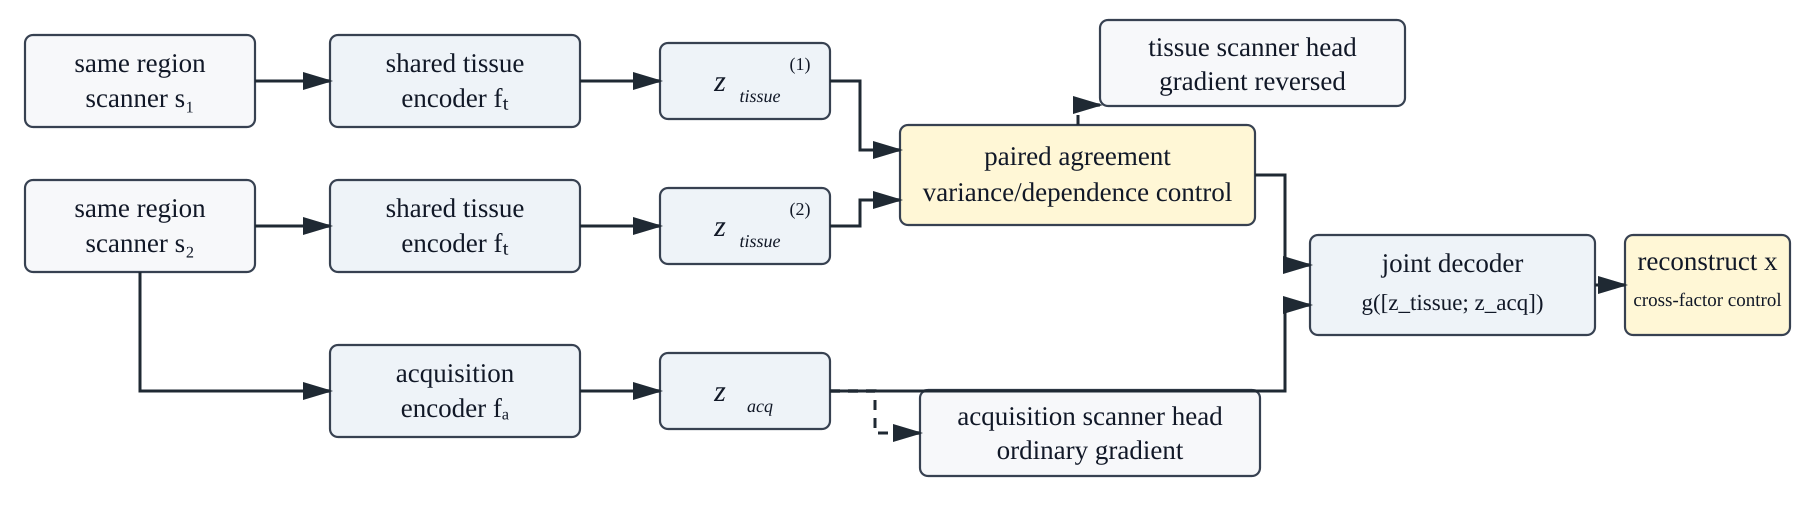
\includegraphics[width=\textwidth]{figures/pa_nf_architecture.pdf}
\caption{Paired-Acquisition Neural Factorization routes matched views of the
same tissue region through a shared tissue-oriented encoder and an explicit
acquisition branch. Paired agreement, variance/dependence control, a
gradient-reversed tissue scanner head, an ordinary acquisition scanner head,
and joint decoding structure how scanner-associated information is allocated.
The diagram describes the implemented architecture; the corrected empirical
boundary remains partial structured separation rather than pure factors,
complete scanner invariance, or clinical utility.}
\label{fig:panf}
\end{figure*}


The representation stage asks whether matched acquisitions can provide a useful supervisory signal for allocating scanner-associated variation without simply erasing the representation. For a region observed under several scanners, PA-NF learns a tissue-oriented branch $b_{r,s}$ and an acquisition-oriented branch $a_{r,s}$, with crossed reconstruction, same-region consistency, acquisition prediction, dependence control, and variance regularization. Tissue or diagnostic category labels are not required to construct the paired objective.

\subsection{Registered SCORPION capacity-matched experiment}
The primary human paired-scanner experiment uses SCORPION \cite{ryu2023scorpion}: 48 original H\&E slides, ten aligned regions per slide, and five scanner views per region, for 480 biological regions and 2,400 images. The registered capacity-matched campaign contains seven variants, five folds, and five seeds, for 175 completed fits. Its primary comparator is an equal-capacity two-branch neural control without the scanner-routing objectives.

\begin{table*}[t]
\centering
\caption{Primary registered SCORPION comparison: PA-NF minus the equal-capacity two-branch neural control. Negative tissue scanner balanced accuracy is favorable; retrieval is judged against the registered 0.02 noninferiority margin.}
\label{tab:scorpion_primary}
\small
\begin{tabular}{lrrl}
\toprule
Metric & Mean difference & 95\% fold/slide interval & Result \\
\midrule
Tissue scanner balanced accuracy & $-0.3108$ & $[-0.3346,-0.2858]$ & Lower scanner recoverability \\
Mean same-region top-1 retrieval & $+0.00004$ & $[-0.00009,+0.00026]$ & Noninferior \\
Mean paired cosine & $+0.03639$ & $[+0.03355,+0.03954]$ & Positive geometry contrast \\
Worst paired cosine & $+0.03557$ & $[+0.03167,+0.04064]$ & Positive geometry contrast \\
Acquisition scanner balanced accuracy & $+0.1180$ & $[+0.1003,+0.1358]$ & Stronger explicit scanner routing \\
\bottomrule
\end{tabular}
\end{table*}

The key result is the joint pattern: tissue-branch scanner recovery falls substantially relative to the capacity-matched neural control, same-region retrieval remains inside the predefined noninferiority margin, and scanner information becomes more recoverable from the acquisition branch. This supports a controlled comparative advantage on the registered SCORPION structured-separation objective. Because SCORPION does not supply a validated biological-category endpoint for these regions, the result is a representation result rather than a disease-biology claim.

\subsection{Cross-backbone transfer}
The frozen objective was transferred without backbone-specific tuning across DINOv2-Base, pathology-native Phikon, and ImageNet ResNet50 representations. In the transfer study, PA-NF reduced scanner recoverability in the tissue branch while retaining near-saturated same-region retrieval across all three feature families. Averaging the two unseen feature families within the same 48 SCORPION slides gave a scanner-probe difference of $-0.4019$ with interval $[-0.4145,-0.3895]$. The acquisition branch remained strongly scanner informative. This result shows that the paired objective is not tied to one visual encoder, although the registered DINOv2 capacity-matched campaign remains the primary controlled comparison.

\subsection{Independent multi-scanner canine SCC study}
The external paired-scanner study uses 44 canine cutaneous squamous-cell-carcinoma biological samples digitized on five scanners. After geometry qualification, 805 complete five-view regions are available. The corrected evaluation fixes five descriptive tissue categories---Dermis, Epidermis, Inflammation/Necrosis, SCC, and Subcutis---and uses biological-sample-blocked folds, fit-only standardization, and same-region/same-sample exclusions in nearest-neighbour candidate pools.

\begin{table*}[t]
\centering
\caption{Corrected five-fold canine SCC representation comparison. Category balanced accuracy is descriptive; lower scanner balanced accuracy and higher retrieval are favorable.}
\label{tab:canine_corrected}
\small
\begin{tabular}{lrrrr}
\toprule
Representation & Category BA & Scanner BA & Overall retrieval & Worst-pair retrieval \\
\midrule
Original frozen features & 0.4439 & 0.8635 & 0.8724 & 0.7613 \\
Centroid/QR scanner projection & 0.4414 & 0.3278 & 0.9099 & 0.8196 \\
Paired linear scanner transform & 0.4422 & 0.3687 & 0.9022 & 0.8283 \\
PCA component removal & 0.3949 & 0.8157 & 0.9197 & 0.8512 \\
PA-NF tissue branch B32 & 0.4331 & 0.2996 & 0.7192 & 0.5848 \\
PA-NF tissue branch B64 & 0.4255 & 0.3486 & 0.7707 & 0.6345 \\
\bottomrule
\end{tabular}
\end{table*}

The canine experiment establishes an important boundary around the SCORPION result. PA-NF B32 attains the lowest mean scanner balanced accuracy in the corrected table, but strong centroid/QR and paired-linear corrections preserve higher retrieval while retaining similar descriptive category accuracy. Under the registered three-axis rule, neither B32 nor B64 establishes a universal neural feature-space increment over every simple baseline. Increasing the tissue bottleneck from 32 to 64 dimensions increases overall retrieval by $+0.0515$ and scanner recoverability by $+0.0489$, while corrected category balanced accuracy changes by $-0.0076$ with an interval crossing zero.

This is not a contradiction with the SCORPION controlled result. The two experiments use different comparators and endpoints. SCORPION establishes a bounded advantage over an equal-capacity neural control on the registered structured-separation objective; the canine study shows that broader scanner correction has a harder frontier in which strong linear methods remain competitive.

\subsection{Pair integrity and information routing}
Broken-pair controls provide a direct test of whether scanner suppression alone explains the result. Region- and sample-shuffled pairings can reduce scanner probe accuracy as much as, or more than, true same-region pairs, but they degrade same-region agreement and retrieval. Correct pairing therefore constrains what the system preserves rather than merely teaching it to confuse a scanner classifier.

The explicit acquisition branch is equally important. Scanner information remains strongly recoverable there, so the intended operation is allocation rather than wholesale deletion. The observed separation is partial and estimator-dependent: low linear scanner recoverability is not information-theoretic independence, and same-region retrieval is not a clinical or diagnostic endpoint.
